\documentclass[12pt]{article}
\usepackage[russian]{babel}
\usepackage[utf8x]{inputenc}
\usepackage{amssymb}
\usepackage{amsmath}
\usepackage{graphicx}
\usepackage{geometry}
\usepackage[colorinlistoftodos]{todonotes}
\usepackage{listings}
\usepackage[section]{placeins}
\begin{document}

\title{5. Оценивание характеристик стационарного случайного процесса}
\author{Андрей Валиков}
\date{}
\maketitle
																																																								\section{Формирование последовательности случайных чисел}
		   																																																						
\[N = 500\]  
	
	  
Параметры случайной функции:
\[b = 1.7\]
\[r(n)= b * \textrm{rand} - \textrm{mean}(r1)\]	


Параметры чистой функции:
\[M1 = 41\]
\[M2 = 23\]
\[f(n)=\sin\left(\frac{2\pi}{M_1}n\right) + \cos\left(\frac{2\pi}{M_2}n\right)\]



\begin{lstlisting}
def F(N):
  M1 = 41
  M2 = 23
  y = np.zeros(N)
  for n in range(N):
    y[n] = np.sin((2 * np.pi * (n - 1)) / M1) + np.cos((2 * np.pi * (n - 1)) / M2)

  return y
  
def R(N):
  b = 1.7
  rl = b * np.random.rand(N)
  k = np.mean(rl)
  y = rl - k
  return y

N = 200
w = np.arange(0, N)

x = F(N)
r = R(N)
y = x + r
\end{lstlisting}

\begin{figure}[!htb]
\centering
%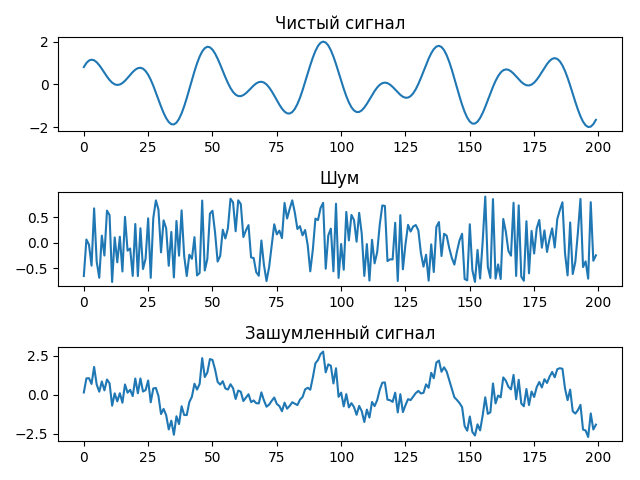
\includegraphics[scale=1.00]{initial.png}
\caption{}
\label{}
\end{figure}


\section{Скользящее среднее}
Формула:

\[y(n + L / 2) = \frac{1}{L + 1}\sum_{\lambda=0}^{L}x(n+\lambda) \]
 


\begin{lstlisting}
def MA(X, L):
  N = len(X)
  y = np.zeros(N)

  for n in range(L // 2 - 1, N - L // 2):
    sum_41 = 0
    for k in range(-L // 2, L // 2):
      sum_41 += X[n + k]
    y[n] = sum_41 / (L + 1)

  return y
\end{lstlisting}



\begin{figure}[!htb]
\centering
%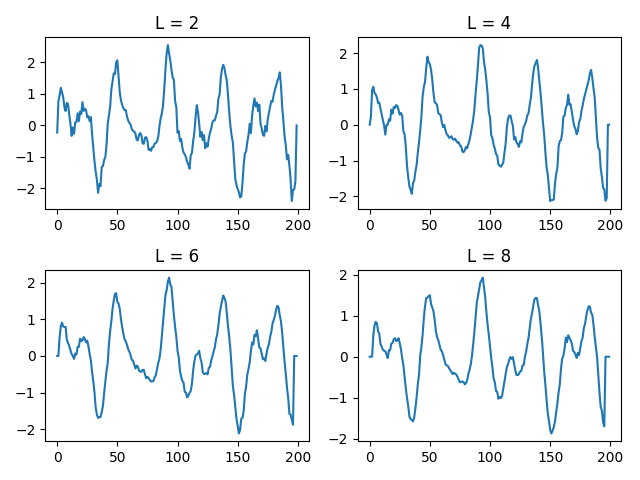
\includegraphics[scale=1.00]{ma.png}
\caption{}
\label{}
\end{figure}

Результат среднеквадратичного отклонения:
\[ 32.844\]
\[ 18.61\]
\[ 15.583\]
\[ 16.063\]

       

\section{Четвёртые разности}

\[y(n) = \frac{1}{35}(-3x(n-2) + 12x(n-1) + 17x(n) + 12x(n+1) - 3x(n+2)) \]

%\[f(\frac{1}{\pi} \int_{0}^{\infty}(\operatorname{Re}(\hat{f})\cos(\omega t) - \operatorname{Im}(\hat{f})\sin(\omega t))d\omega \]

\begin{lstlisting}
def MoFD(X):
  N = len(X)
  y = np.zeros(N)
  for n in range(2, N - 2):
    y[n] = (-3 * X[n - 2] + 12 * X[n - 1] + 17 * X[n] + 12 * X[n + 1] - 3 * X[n + 2]) / 35

  return y
\end{lstlisting}

Среднеквадратичное отклонение 22.855.

\begin{figure}[!htb]
\centering
%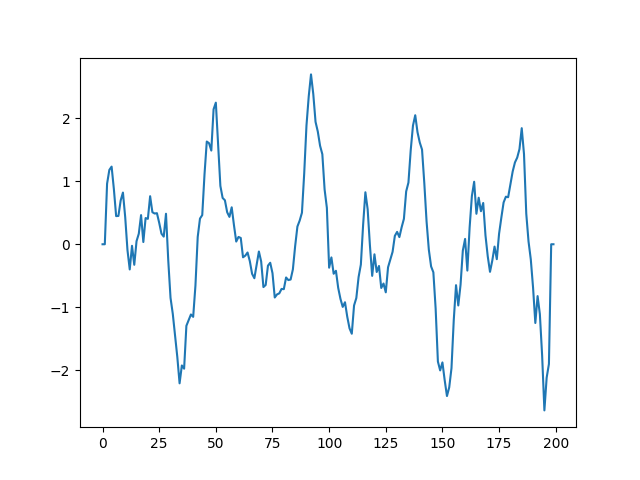
\includegraphics[scale=1.00]{fourth_diff.png}
\caption{}
\label{}


\end{figure}

\section{Экспоненциальное сглаживание}
\[y(n) = \alpha \sum_{\nu=0}^{n-1}(1-\alpha)^\nu x(n-v) + (1 - \alpha)^n x(0) \]
Значения a и соответствующие значения среднеквадратичного отклонения: \\
0.1 : 124.0\\
0.2 : 68.0\\
0.3 : 39.0\\
0.4 : 26.0\\
0.5 : 21.0\\
0.6 : 21.0\\
0.7 : 23.0\\
0.8 : 27.0\\
0.9 : 32.0\\
\begin{figure}[htp]
\centering
%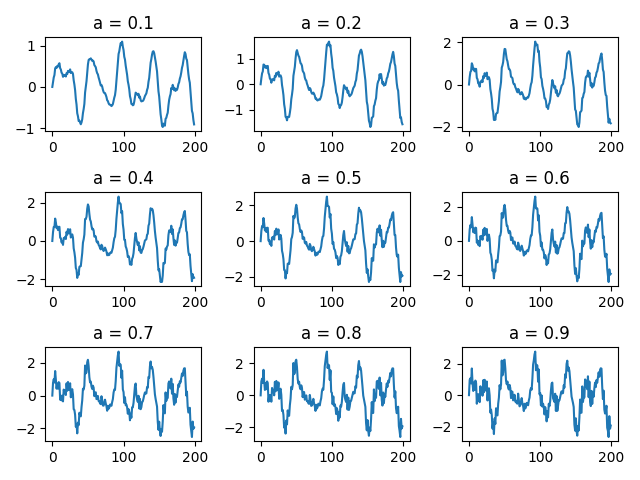
\includegraphics[scale=1.00]{exp.png}
\caption{}
\label{}
\end{figure}

\section{Вывод}
Рассмотрена задача о сглаживании дискретной последовательности, состоящей из чистого сигнала и зашумления. Сглаживание позволяет устранить влияние помехи на сигнал. В данной работе были реализованы три метода сглаживания: скользящее среднее, метод четвертых разностей и экспоненциальный метод. Чем ниже значение, получаемое на выходе, тем качественнее сглаживание.\\
Последовательность задаётся как совокупность помехи и полезного сигнала, после чего данная последовательность сглаживается методами, описанными выше.
Качество сглаживания оценивалось с помощью метода наименьших квадратов.
Лучшие показатели сглаживания используемых методов при различном значении параметров:\\
Скользящее среднее: L = 6: 11.478\\
Метод четвертых разностей (без параметров): 22.855\\
Экспоненциальный метод: a = 0.5, 0.6: 21\\
В результате проведенных испытаний и полученных результатов показателей качества сглаживания, можно сделать вывод о том, что сглаживание скользящим средним дает наилучший показатель.

\end{document}